\section{Implementation}\label{sec:implem}

The core of YETI is an application coded in Java, allowing to test programs at random in a fully automated manner. It is designed to support various programming languages -- for example, functional, procedural and object-oriented languages can easily be supported.
 It contains three parts: the core infrastructure, the strategy, and the language-specific bindings. 
YETI is a lightweight platform with around 5000 lines of code for the core, graphical interfaces and the strategies.
The .NET binding in itself consists of around 1000 lines of code in Java and 1700 lines of code in C\#.

\subsection{Using YETI}
YETI is a tool that can be launched on the command-line. A typical call of YETI that tests .NET assemblies is:
{\small
\begin{verbatim}
java yeti.Yeti -dotnet -time=10mn -randomPlus
-testModules=Assembly1.dll:Assembly2.dll
\end{verbatim}
}

The options used on this command-line have the following meaning: \texttt{-dotnet} 
indicates that the tested program is in .NET bytecode,
\texttt{-time=10mn} indicates that the testing session will last 10 minutes, 
\texttt{-randomPlus} indicates that the strategy random+ will be used, and  
\texttt{-testModules=Assembly1.dll:Assembly2.dll} indicates that both \texttt{Assembly1.dll} and
\texttt{Assembly2.dll} will be tested.

While testing, traces of faults found are output in the terminal. For example:

{\small
\begin{verbatim}
Exception 15
	Value cannot be null.
Parameter name: to
   at System.Net.Mail.MailMessage..ctor(String 
             from, String to)
   at System.Net.Mail.MailMessage..ctor(String 
             from, String to, String subject, 
             String body)
\end{verbatim}
}

At the end of the testing sessions, YETI outputs generated test cases reproducing 
the faults found during the testing session as well.


Note that it is also possible to avoid the overhead of keeping the 
traces in the system (and calculating the minimal test cases) by specifying 
\texttt{-nologs} to throw away all logs except exception traces, or 
\texttt{-rawlogs} to output the logs to the terminal.

\subsection{Graphical User Interface (GUI)}
By specifying the \texttt{-gui} option, YETI shows a graphical user interface
that allows test engineers to interact directly with the system while the testing 
session proceeds. 

\begin{figure*}[h!]
\begin{center}
\begin{sideways}
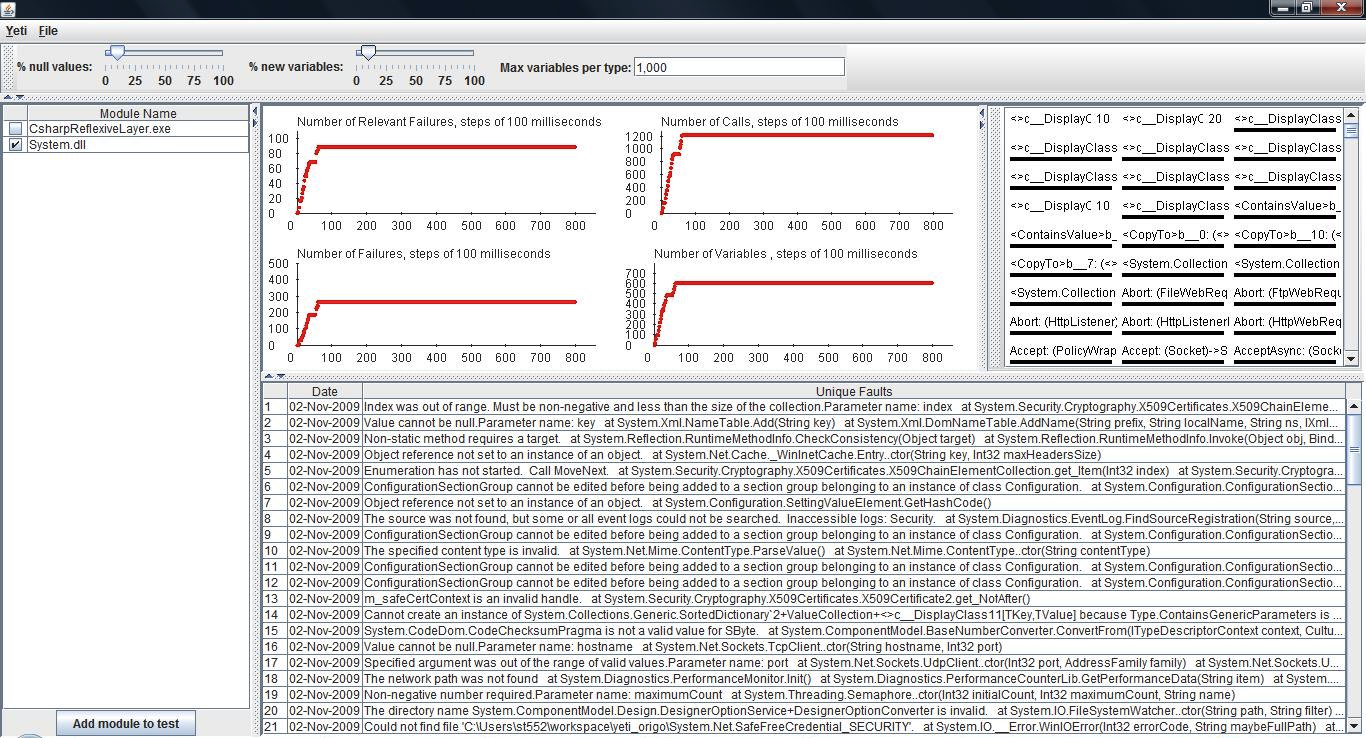
\includegraphics[width=24cm]{images/ScreenShotdotNET.png}
\end{sideways}
\end{center}
\caption{YETI graphical user interface.}\label{fig:gui}
\end{figure*}


Figure~\ref{fig:gui} shows YETI's graphical user interface when using 
the random strategy. At the top of the interface, two sliders correspond to 
the percentage of null values and the percentage of new variables to use when testing.
In short, each time a test is made, each parameter of the routine to test can either 
be void, be newly generated or a new variable. These sliders indicate which probability 
to use. In the top part there is also a text field to limit the number of instances per 
type in the system (which is necessary for long-running sessions).

The left panel contains a list of modules loaded in 
the system. The modules being tested are ticked, while others can be used as helpers to 
create variables to use on-demand making a routine calls. A button is available to add modules 
at runtime for programming languages that support it. This last part is useful in cases 
where a module is missing to enable the testing of a routine. 

In the central panel, four graphs describe the evolution of the system: the top-left one shows 
the evolution of the number of unique failures found -- all failures without redundancy --, the 
bottom-left indicates the raw number of failures over time, the bottom-right indicates the current 
number of instances in the system, the top-right panel indicates the total number of calls effected by YETI.

The panel on the right shows all methods tested in the system.

The bottom panel reports unique failures as they are found: each line is a unique failure.

In order for the graphical interface not to slow down the testing process, we use two threads.
The first one samples data for building graphs every .1 seconds, the second one updates the graphical user interfaces and waits .1 second between two updates. A special care has also been taken for not showing all samples in the graphs when not needed: we only show one point per pixel on the x-axis.

\subsection{Core Architecture}
The core architecture of YETI is very consistent with the model described in Section~\ref{sec:model}.
YETI uses the core notions of types, routine, modules and variables by defining respectively Java classes 
\texttt{YetiType}, \texttt{YetiRoutine}, \texttt{YetiModule}, and \texttt{YetiVariable}.
YETI also maintains the types constraints as discussed in Section 2.

\begin{figure}[h]
\begin{center}
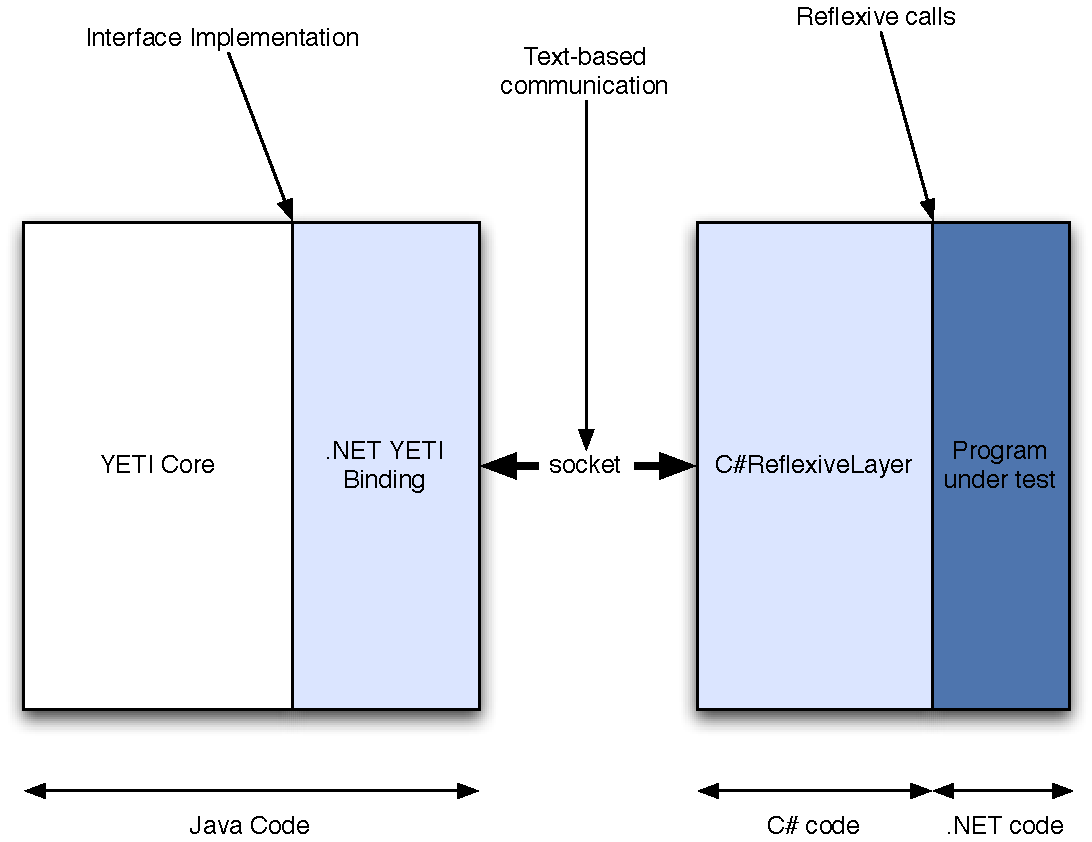
\includegraphics[width=\columnwidth]{images/Architecture.pdf}
\end{center}
\caption{Yeti .NET binding architecture.}\label{fig:archi}
\end{figure}

Extending YETI to support a new programming language is done through specializing a set of abstract classes in the YETI core.
In the case of the .NET binding, it was necessary to make the Java language-agnostic part communicate with the .NET code through a custom-made communication layer. We chose to use a socket-based solution for its modularity and potential for distributed testing sessions.

Figure~\ref{fig:archi} shows the main structure of the YETI .NET binding. The architecture consists of three main different parts: 
\begin{itemize}
\item the main YETI core in white,
\item the .NET binding in light blue,
\item the program under test in dark blue.
\end{itemize} 

The .NET binding itself is coded both in Java and C\#. The C\# part is the C\#ReflexiveLayer is a very simple text-based interpreter for extracting information from the .NET code under test, making calls of routines in the program under test, maintaining a variable pool and returning results. The Java part is a simple stub between standard YETI structure and the interpreter. 

The communication between the two parts of the .NET binding is text-based.
When first loaded the C\# reflexive layer queries all information in loaded assemblies and sends it to the YETI part. This constitutes the initialization of the .NET binding.
Then the Java part of the binding translates method calls ordered
by the main YETI infrastructure in a text-based, sends them through the socket 
and reads the result of the computation. The C\# reflexive layer performs the calls 
and returns the results, be it an exception trace, a newly created variable or only the indication of no failure.

The failures are stored in the core Java part and the logs are processed in the binding's Java part at the end of the testing session.

